
回到上一章讨论的主题,从设置安装和打包所需文件的快速概述开始:

\begin{center}
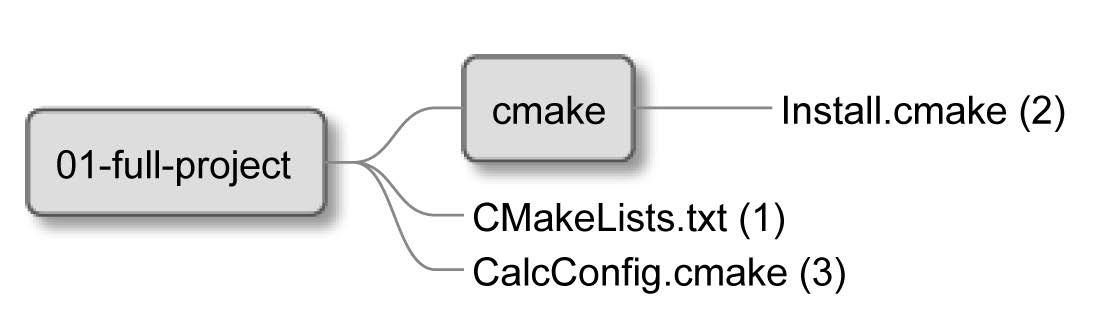
\includegraphics[width=0.6\textwidth]{content/3/chapter12/images/6.jpg}\\
图12.6 配置安装和打包的文件
\end{center}

这里只需要文件——大部分工作已经在前面的小节中完成了。顶层的列表文件包括一个CMake模块,将处理这个过程:

\begin{lstlisting}[style=styleCMake]
# chapter-12/01-full-project/CMakeLists.txt (fragment)

...
include(Install)
\end{lstlisting}

我们有兴趣安装两个项目:

\begin{itemize}
\item 
Calc库构件:静态库、动态库、头文件,以及目标导出的文件

\item 
Calc控制台可执行文件
\end{itemize}

包定义配置文件将只引入库目标,因为潜在的使用项目不会依赖于可执行文件。

配置安装步骤之后,将继续进行CPack配置。Install模块的概述如下:

\begin{lstlisting}[style=styleCMake]
# chapter-12/01-full-project/cmake/Install.cmake (overview)

# Includes
# Installation of Calc library
# Installation of Calc Console executable
# Configuration of CPack
\end{lstlisting}

一切都计划好了,所以是时候为库编写安装模块了。

\subsubsubsection{12.6.1\hspace{0.2cm}库的安装}

安装库最好从配置逻辑目标,并为其工件指定目的地开始。为了避免手动提供路径,将使用GNUInstallDirs模块提供的默认值。为了模块化,将把构件分组到组件中。默认安装将安装所有文件,可以选择只安装运行时组件,而跳过开发构件:

\begin{lstlisting}[style=styleCMake]
# chapter-12/01-full-project/cmake/Install.cmake (fragment)

include(GNUInstallDirs)
# Calc library
install(TARGETS calc_obj calc_shared calc_static
	EXPORT CalcLibrary
	ARCHIVE COMPONENT development
	LIBRARY COMPONENT runtime
	PUBLIC_HEADER DESTINATION
		${CMAKE_INSTALL_INCLUDEDIR}/calc
			COMPONENT runtime
)
\end{lstlisting}

安装过程中,我们想用ldconfig注册复制的动态库:

\begin{lstlisting}[style=styleCMake]
# chapter-12/01-full-project/cmake/Install.cmake (continued)

if (UNIX)
	install(CODE "execute_process(COMMAND ldconfig)"
		COMPONENT runtime
	)
endif()
\end{lstlisting}

准备好这些步骤后,就可以通过将库包装在可重用的CMake包中,使它对其他CMake项目可见。需要生成并安装目标导出文件和包含它的配置文件:

\begin{lstlisting}[style=styleCMake]
# chapter-12/01-full-project/cmake/Install.cmake (continued)

install(EXPORT CalcLibrary
	DESTINATION ${CMAKE_INSTALL_LIBDIR}/calc/cmake
	NAMESPACE Calc::
	COMPONENT runtime
)
install(FILES "CalcConfig.cmake"
	DESTINATION ${CMAKE_INSTALL_LIBDIR}/calc/cmake
)
\end{lstlisting}

对于非常简单的包,配置文件可以非常小:

\begin{lstlisting}[style=styleCMake]
# chapter-12/01-full-project/CalcConfig.cmake\\

include("${CMAKE_CURRENT_LIST_DIR}/CalcLibrary.cmake")
\end{lstlisting}

现在,当构建解决方案后可以以-{}-install模式运行cmake,将安装该库。剩下要安装的就是可执行文件了。

\subsubsubsection{12.6.2\hspace{0.2cm}可执行文件的安装}

安装二进制可执行程序是所有步骤中最简单的步骤,只需要使用一个命令:

\begin{lstlisting}[style=styleCMake]
# chapter-12/01-full-project/cmake/Install.cmake (continued)

# CalcConsole runtime
install(TARGETS calc_console
	RUNTIME COMPONENT runtime
)
\end{lstlisting}

完成了!现在来到了配置的最后一步——打包。

\subsubsubsection{12.6.3\hspace{0.2cm}使用CPack打包}

这时,就可以随心所欲地配置受支持的包类型。然而,对于这个项目,基本配置就足够了:

\begin{lstlisting}[style=styleCMake]
# chapter-12/01-full-project/cmake/Install.cmake (continued)

# CPack configuration
set(CPACK_PACKAGE_VENDOR "Rafal Swidzinski")
set(CPACK_PACKAGE_CONTACT "email@example.com")
set(CPACK_PACKAGE_DESCRIPTION "Simple Calculator")
include(CPack)
\end{lstlisting}

这种最小的设置适用于标准档案,例如ZIP文件。可以用一个命令来测试整个安装和打包(项目必须事先构建):

\begin{tcblisting}{commandshell={}}
# cpack -G TGZ -B packages
CPack: Create package using TGZ
CPack: Install projects
CPack: - Run preinstall target for: Calc
CPack: - Install project: Calc []
CPack: Create package
CPack: - package: /tmp/b/packages/Calc-1.0.0-Linux.tar.gz
generated.
\end{tcblisting}

这就结束了安装和包装,下一个任务是生成文档。










